\documentclass[12pt,xcolor={table},aspectratio=169]{beamer}



\usetheme{BUAA}
\usepackage{thumbpdf}
\usepackage{wasysym}
% \usepackage{ucs}
\usepackage[utf8]{inputenc}
\usepackage{pgf,pgfarrows,pgfnodes,pgfautomata,pgfheaps,pgfshade}
\usepackage{pgfplotstable}
\usepackage{verbatim}
\usepackage{xeCJK}
\usepackage{amsmath,amssymb,amsfonts,mathrsfs,bm}
\usepackage{siunitx,booktabs}
\usepackage{pgfplots}
\usepackage{array}
\usepackage{multirow}
\usepackage{setspace}
\pgfplotsset{compat=1.13}
%\sisetup{load-configurations = abbreviations}

\usetikzlibrary{shapes.arrows,decorations.pathmorphing,backgrounds,fit,positioning,shapes.symbols,chains}
\usetikzlibrary{spy}
\usetikzlibrary{calc,fadings,decorations.pathreplacing}
\usetikzlibrary{intersections,decorations.markings}
\usetikzlibrary{angles}
\usetikzlibrary{quotes}


\usepackage{mathtools}
\newcommand{\defeq}{\vcentcolon=}
\newcommand{\eqdef}{=\vcentcolon}

\newcommand{\RNum}[1]{\uppercase\expandafter{\romannumeral #1\relax}}


% \mathnormal{3x^2 \in R \subset Q} \\
% \mathrm{3x^2 \in R \subset Q} \\
% \mathit{3x^2 \in R \subset Q} \\
% \mathbf{3x^2 \in R \subset Q} \\
% \mathsf{3x^2 \in R \subset Q} \\
% \mathtt{3x^2 \in R \subset Q}
% \mathcal{RQSZ} \\
% \mathfrak{RQSZ} \\
% \mathbb{RQSZ}
% \operatorname

\title[title-short]{标题标题标题标题Title标题标题标题\\长标题长标题长标题长标题}
\subtitle{副标题副标题Subtitle副标题副标题}
\author[Htallone et al.]{Htallone\inst{1} \and 作者 X\inst{2}}%
\institute[BUAA]
{
  \inst{1}%
  北京航空航天大学 \ 宇航学院
  \and%
  \inst{2}%
  XXXXXXX
}

\renewcommand{\today}{\number\year 年\number\month 月\number\day 日}%
\date[]{\CJKsetecglue{}\today}
%\date{\CJKsetecglue{}{2016年6月7日}}
% \date{\small 20 November, 2017}

\newcommand{\head}[1]{\textnormal{\textbf{#1}}}
\newtheorem*{remark}{Remark}
\DeclareMathOperator*{\argmin}{arg\,min}

%%%%%%%%%%%%%%%%%%%%%%%%%%%%%%

\pgfdeclareradialshading{ballshading}{\pgfpoint{-10bp}{10bp}}%
 {%
 color(0bp)=(gray!10!white);
 color(15bp)=(gray!20!white);
 color(25bp)=(gray!70!black);
 color(35bp)=(gray!50!black);
 color(50bp)=(black!70)}%



\makeatletter
\patchcmd{\beamer@sectionintoc}{\vskip1.5em}{\vskip0.5em}{}{}
\makeatother
\usepackage{calligra}





\begin{document}

\newcommand<>{\highlighton}[1]{%
  \alt#2{\structure{#1}}{{#1}}
}
\newcommand{\highlightmath}[2][yellow]{\mathchoice%
  {\colorbox{#1}{$\displaystyle#2$}}%
  {\colorbox{#1}{$\textstyle#2$}}%
  {\colorbox{#1}{$\scriptstyle#2$}}%
  {\colorbox{#1}{$\scriptscriptstyle#2$}}}%

\newcommand{\icon}[1]{\pgfimage[height=1em]{#1}}

\newcommand\abs[1]{\left|#1\right|}

\newlength\dlf
\newcommand\alignedbox[3][yellow]{
  % #1 = color (optional, defaults to yellow)
  % #2 = before alignment
  % #3 = after alignment
  &
  \begingroup
  \settowidth\dlf{$\displaystyle #2$}
  \addtolength\dlf{\fboxsep+\fboxrule}
  \hspace{-\dlf}
  \fcolorbox{#1}{#1}{$\displaystyle #2 #3$}
  \endgroup
}



%%%%%%%%%%%%%%%%%%%%%%%%%%%%%%%%%%%%%%%%%
%%%%%%%%%% Content starts here %%%%%%%%%%
%%%%%%%%%%%%%%%%%%%%%%%%%%%%%%%%%%%%%%%%%

\begin{frame}[plain]
    \titlepage
\end{frame}

\section*{目录}
\begin{frame}
  \frametitle{目录}
  \tableofcontents[hidesubsections]
\end{frame}

\section{引言}
\begin{frame}
  \frametitle{引言:伴随法}
  \vskip-2em
  \emph{伴随法},又称为伴随仿真技术, is a useful computerized tool for the analysis of \emph{linear time-varying systems}.\\[2ex]
  
  With the adjoint method, \emph{error budgets} or sensitivities of the LTV system due to all disturbance input terms can be automatically generated.\\[2ex]
  
  In this paper, new interpretations of the adjoint method are achieved by using the \emph{adjoint definition equation
  } in state-space form.
\end{frame}


\begin{frame}
  \frametitle{引言:伴随概念}
  \vskip-1em
Suppose $\bm{G} : \mathcal{U} \mapsto \mathcal{Y}$ is a linear system,  $\mathcal{U}$ and $\mathcal{Y}$ are Hilbert spaces. The adjoint of $\bm{G}$ is the linear system $\bm{G}^* : \mathcal{Y} \mapsto \mathcal{U}$ such that 
\begin{equation}
\label{eqnAdjointDef}
\langle \bm{G}u,y \rangle_{\mathcal{Y}} = \langle u,\bm{G}^* y \rangle_{\mathcal{U}}   \quad \forall u\in \mathcal{U},\ \forall y\in \mathcal{Y},
\end{equation}
where $\langle \cdot,\cdot \rangle$ denotes the \emph{inner product} defined by
\begin{equation}
\label{eqnInnerProduct}
\langle f,g \rangle = \int_{t_0}^{t_{\mathrm{f}}} g^{\mathrm{T}}(t) f(t) \mathrm{d}t, \quad f,g \in \mathcal{U}\ \text{or} \ \mathcal{Y} 
\end{equation}
\begin{equation}
\label{eqnGenInnerProduct}
\langle \begin{bmatrix}
f_0\\
f
\end{bmatrix},\begin{bmatrix}
g_0\\
g
\end{bmatrix} \rangle = g_0^{\mathrm{T}}f_0 + \int_{t_0}^{t_{\mathrm{f}}} g^{\mathrm{T}}(t) f(t) \mathrm{d}t,
\quad \begin{bmatrix}
f_0\\
f
\end{bmatrix}, \begin{bmatrix}
g_0\\
g
\end{bmatrix} \in \mathbb{R}^n \oplus \mathcal{U}\ \text{or}\ \mathbb{R}^n \oplus \mathcal{Y}
\end{equation}

\end{frame}

\section[伴随系统]{伴随系统状态空间描述}
  
  \begin{frame}
    \frametitle{伴随定义方程}
    \vspace{-1em}
\begin{equation}
\footnotesize
\highlightmath{
p^{\mathrm{T}}(t_{\mathrm{f}})x(t_{\mathrm{f}}) - p^{\mathrm{T}}(0)x(0)= \int_{0}^{t_{\mathrm{f}}} -r^{\mathrm{T}}(t)y(t)+ u^{\mathrm{T}}(t)q(t) \mathrm{d}t.}
\end{equation}
      \vspace{-2em}
    \begin{columns}
    \begin{column}[t]{0.4\paperwidth}
  \begin{block}{线性系统}
  {\setlength\abovedisplayskip{1pt}
  \setlength\belowdisplayskip{1pt}
  \begin{equation}
 \bm{G} : \mathbb{R}^n \oplus \mathcal{U} \mapsto \mathbb{R}^n \oplus \mathcal{Y}; \begin{bmatrix}
x_0\\
u
\end{bmatrix}
\mapsto
\begin{bmatrix}
x_{\mathrm{f}}\\
y
\end{bmatrix} 
  \end{equation}
   }%
  \end{block}
  \end{column}
      \begin{column}[t]{0.4\paperwidth}
  \begin{block}{伴随系统}
  {\setlength\abovedisplayskip{1pt}
  \setlength\belowdisplayskip{1pt}
    \begin{equation}
 \bm{G}^* : \mathbb{R}^n \oplus \mathcal{Y} \mapsto \mathbb{R}^n \oplus \mathcal{U}; \begin{bmatrix}
p_{\mathrm{f}}\\
r
\end{bmatrix}
\mapsto
\begin{bmatrix}
p_0\\
q
\end{bmatrix}
  \end{equation}
  }%
  \end{block}
  \end{column}
  \end{columns}
  \vspace{0.5em}
  \begin{equation}
  \footnotesize
\left\langle \bm{G}\begin{bmatrix}
x_0\\
u
\end{bmatrix},\begin{bmatrix}
p_{\mathrm{f}}\\
r
\end{bmatrix} \right\rangle_{\mathbb{R}^n \oplus \mathcal{Y}} = \left\langle \begin{bmatrix}
x_0\\
u
\end{bmatrix},\bm{G}^* \begin{bmatrix}
p_{\mathrm{f}}\\
r
\end{bmatrix} \right\rangle_{\mathbb{R}^n \oplus \mathcal{U}}   \quad \forall \begin{bmatrix}
x_0\\
u
\end{bmatrix}\in \mathbb{R}^n \oplus \mathcal{U},\ \forall \begin{bmatrix}
p_{\mathrm{f}}\\
r
\end{bmatrix}\in \mathbb{R}^n \oplus \mathcal{Y},
\end{equation}
  
  \begin{equation}
  \footnotesize
\left\langle \begin{bmatrix}
f_0\\
f
\end{bmatrix},\begin{bmatrix}
g_0\\
g
\end{bmatrix} \right\rangle = g_0^{\mathrm{T}}f_0 + \int_{t_0}^{t_{\mathrm{f}}} g^{\mathrm{T}}(t) f(t) \mathrm{d}t.
\end{equation}
  
  \end{frame}
  
\begin{frame}
    \frametitle{伴随系统总结}
        \vspace{0em}
    \begin{columns}
    \begin{column}[c]{0.4\paperwidth}
  \begin{block}{线性系统}
  {\setlength\abovedisplayskip{1pt}
  \setlength\belowdisplayskip{1pt}
\begin{equation*}
\left .
 \begin{aligned}
        \dot{x}(t) &= A(t)x(t)+B(t)u(t), \\
        y(t) & = C(t)x(t)+D(t)u(t)
 \end{aligned} \right \}
\end{equation*}
   }%
  \end{block}
    \begin{block}{伴随系统}
  {\setlength\abovedisplayskip{1pt}
  \setlength\belowdisplayskip{1pt}
\begin{equation*}
\left .
  \begin{aligned}
        \dot{z}(t) &= A^{\mathrm{T}}(t_{\mathrm{f}}-t)z(t)+C^{\mathrm{T}}(t_{\mathrm{f}}-t)v(t),  \\
        w(t) & = B^{\mathrm{T}}(t_{\mathrm{f}}-t)z(t)+D^{\mathrm{T}}(t_{\mathrm{f}}-t)v(t)
 \end{aligned} \right \}
\end{equation*}
  }%
  \end{block}
  \end{column}
      \begin{column}[c]{0.4\paperwidth}
      \vspace{0.5em}
        \begin{minipage}[c][0.6\textheight][c]{\linewidth}
    \centering
\begin{figure}
    \centering
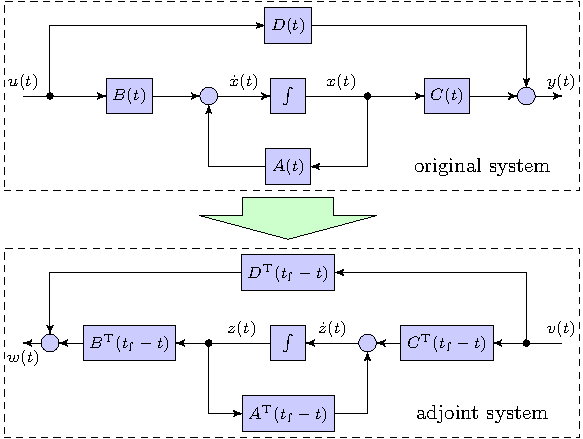
\includegraphics[scale=0.6]{image/adjCnstr}
% \caption{Adjoint system construction}
\end{figure}
\end{minipage}
  \end{column}
  \end{columns}
    \footnotesize
\begin{equation}
\highlightmath{
z^{\mathrm{T}}(0)x(t_{\mathrm{f}}) - z^{\mathrm{T}}(t_{\mathrm{f}})x(0) = \int_{0}^{t_{\mathrm{f}}} -v^{\mathrm{T}}(t_{\mathrm{f}} - t)y(t)+ u^{\mathrm{T}}(t)w(t_{\mathrm{f}}-t) \mathrm{d}t }
\end{equation}
\end{frame}

\section[结论]{结\quad 论}
\begin{frame}
    \frametitle{结\quad 论}
    \begin{itemize}
  \setlength{\itemsep}{10pt}
    \item The interpretation of adjoint simulation was achieved in a new and universal way, by using the adjoint definition equation in state-space form;
    \item The adjoint technique in covariance analysis was also derived;
    \item The adjoint concept is fundamental in mathematics, and naturally arises or is widely used in optimization, optimal control, stability analysis, navigation problems, circuit analysis, etc.
  \end{itemize}

\end{frame}




\frame{
  \vspace{1.5cm}
  {\huge Thank You!}
  
 \vspace{1cm}
  {\qquad \qquad \qquad \qquad \qquad \quad \quad \huge Questions?}

  \vspace{1.2cm}
  \begin{flushright}
    Htallone

    \structure{\footnotesize{Email: Htallone@buaa.edu.cn}}
  \end{flushright}
}


\section[附录]{附录}


\frame[noframenumbering]{
  \vfill
  \centering
  {\huge 附 \quad 录 }
  \vfill
}


\begin{frame}[noframenumbering]
    \frametitle{Basic Definitions and Properties of LTV}
    \tiny
Consider the linear system 
\begin{equation}
\label{eqnLinearSystemAbs}
\begin{aligned}
 \bm{G} &: \mathcal{U} \mapsto \mathcal{Y}\\
  & : u \mapsto y = \bm{G}u,
\end{aligned}
\end{equation}
described by state-space equations
\begin{equation}
\label{eqnStateSpace}
 \begin{aligned}
        \dot{x}(t) &= A(t)x(t)+B(t)u(t), \quad x(t_0) = x_0 \in \mathbb{R}^n \\
        y(t) & = C(t)x(t)+D(t)u(t).
 \end{aligned}
\end{equation}
We are primarily concerned with the linear system $\bm{G}$ in the finite-horizon case. In (\ref{eqnLinearSystemAbs}), $\mathcal{U}$ and $\mathcal{Y}$ are finite-horizon Lebesgue 2-spaces $\mathcal{L}_2[t_0, t_{\mathrm{f}}]$, and $u \in \mathcal{U}$, $y \in \mathcal{Y}$.
In (\ref{eqnStateSpace}), $u(t)\in \mathbb{R}^m$ is the input vector, $x(t)\in \mathbb{R}^n$ is the state vector, $y(t)\in \mathbb{R}^p$ is the output vector; $A(t)$, $B(t)$, $C(t)$ and $D(t)$ are continuous real matrix valued functions of time with appropriate dimensions.

Let $\Phi(t,\tau)$ be the \emph{state transition matrix} associated with system (\ref{eqnStateSpace}), which has the following properties
%       & \Phi(t_2,t_0) = \Phi(t_2,t_1)\Phi(t_1,t_0), \label{eqnSTMp4}
\begin{subequations} \label{eqnSTM}
     \begin{align}
      & \dfrac{\mathrm{d}}{\mathrm{d}t} \Phi(t,\tau) =  A(t)\Phi(t,\tau),\ \Phi(\tau,\tau) = I, \label{eqnSTMp1}\\
      & \Phi^{-1}(t,\tau) = \Phi(\tau,t), \label{eqnSTMp3}
     \end{align}
\end{subequations}
in which $I$ denotes the identity matrix. 
Then the solution to (\ref{eqnStateSpace}) is
\begin{subequations} \label{eqnSolution}
     \begin{align}
      & x(t) = \Phi(t,t_0)x(t_0) + \int_{t_0}^{t} \Phi(t,\tau) B(\tau)u(\tau) \mathrm{d}\tau, \label{eqnSolution1}\\
      & y(t) = C(t)\Phi(t,t_0)x(t_0) + \int_{t_0}^{t} C(t)\Phi(t,\tau) B(\tau)u(\tau) \mathrm{d}\tau + D(t)u(t).\label{eqnSolution2} 
     \end{align}
\end{subequations}
In (\ref{eqnSolution2}), the first term is known as the \emph{zero-input response}, the other terms the \emph{zero-state response}. The zero-state response may be represented by the integral operator
\begin{equation}
\label{eqnImpulseRF}
y(t) = \int_{t_0}^{t_{\mathrm{f}}} H(t,\tau) u(\tau) \mathrm{d}\tau,
\end{equation}
in which 
\begin{equation}
\label{eqnImpulseRFSS}
    H(t,\tau)= 
\begin{cases}
    C(t)\Phi(t,\tau) B(\tau)+D(t)\delta(t-\tau),& \text{if } t\geq \tau\\
    0,              & \text{otherwise}
\end{cases}
\end{equation}
\end{frame}



\begin{frame}[noframenumbering]
    \frametitle{Construction Rules for Adjoint System}
    \vspace{0em}
    \begin{columns}
\begin{column}[c]{0.57\paperwidth}
      \vspace{0.5em}
        \begin{minipage}[c][0.8\textheight][c]{\linewidth}
    \centering
\begin{figure}
    \centering
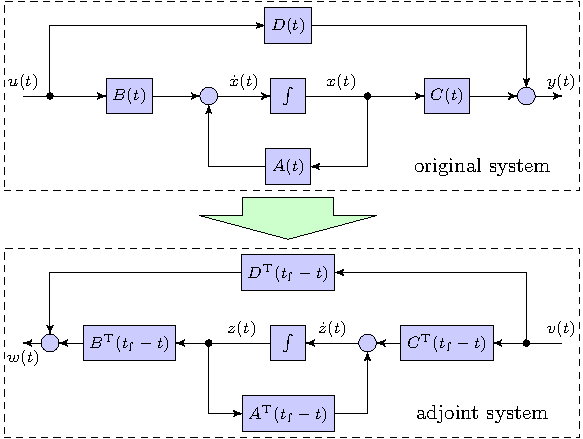
\includegraphics[scale=0.8]{image/adjCnstr}
\caption{Construction of adjoint system from original system}
\label{figLabelAdjointConstruct}
\end{figure}
\end{minipage}
  \end{column}
      \begin{column}[c]{0.37\paperwidth}
      \vspace{0.5em}
        \begin{minipage}[c][0.8\textheight][c]{\linewidth}
    \centering
    \footnotesize
The block diagrams of the orignal system and the adjoint system are shown in Figure. \ref{figLabelAdjointConstruct}, which can be used to explain the general construction rules [Laning; Zarchan; Yanushevsky] of an adjoint system from the orignal system:
\begin{enumerate}
\item Replace $t$ by $t_{\mathrm{f}}-t$ in the arguments of all variable coefficients where $t_{\mathrm{f}}$ is the final time.
\item Reverse all signal flow, redefine branch points ($\vcenter{\hbox{
\includegraphics[scale=0.9]{image/takeoff}}}$) as sum points ($\vcenter{\hbox{
\includegraphics[scale=0.9]{image/sum}}}$), and vice versa.
\end{enumerate}
\end{minipage}
  \end{column}
  \end{columns}

\end{frame}



\end{document}
